\documentclass[a4paper,12pt,catalan]{book}

\usepackage[utf8]{inputenc}
\usepackage[catalan]{babel}
\usepackage{biblatex} % [backend=biber]
\bibliography{bibliografia/memoria}
\usepackage{graphicx}
\usepackage{setspace}
\usepackage{times}
\usepackage{hyperref}
\usepackage{algorithm}
\usepackage{algpseudocode}
\usepackage{caption}

\DeclareCaptionType{mycapequ}[][Llistat d'equacions]
\captionsetup[mycapequ]{labelformat=empty}

%\usepackage{geometry}
%\geometry{verbose,a4paper,tmargin=25mm,bmargin=25mm,lmargin=3cm,rmargin=2cm}

\spacing{1.3}
\AtBeginDocument{\let~=\nobreakspace}

\makeatother

\begin{document}

\pagenumbering{roman}

\pagestyle{plain}
\thispagestyle{empty}

\vspace{0.39cm}
\begin{flushright}
\includegraphics[width=\textwidth]{figs/logos.png}
\end{flushright}
\vspace{0.39cm}

\vfill{}

{\par\centering \textsc{\Large Plataforma eMovie: Xarxa social de pel·lícules}\par}
\vfill{}

\begin{flushright}
\begin{minipage}[b]{0.5\textwidth}

Memòria del projecte d'Enginyeria en Informàtica realitzat per Roger Llopart Pla i dirigit per Jordi Gonzàlez i Sabaté.\\

Bellaterra, 16 de setembre de 2013
\end{minipage}
\end{flushright}
\vfill{}

\cleardoublepage
\vspace*{6 true cm} \begin{center} \begin{minipage}{4in}
\parindent=0pt El firmant, Jordi Gonzàlez i Sabaté, professor del Departament d'Enginyeria de la Informació i de les Comunicacions de la Universitat Autònoma de Barcelona \\

CERTIFICA:\\

Que la present memòria ha estat realitzada sota la seva direcció per
Roger Llopart Pla \par \vspace*{.5in} Bellaterra, 16 de setembre de 2013
\vspace*{.5in}
\begin{center} \vrule width 3in height 0.4pt\\Firmat: Jordi Gonzàlez i Sabaté
\end{center} \end{minipage} \end{center}


\chapter*{Agraïments}

Voldria agraïr a tothom que m'ha ajudat amb aquest projecte. Especial menció al meu tutor del projecte, Jordi Gonzàlez i Sabaté, per tota l'ajuda que m'ha brindat. També mencionar a les comunitats de Mahout i Movielens, el treball de les quals ha estat inestimable per a la realització d'aquest projecte.

\tableofcontents

\newpage
\pagenumbering{arabic}
\pagestyle{headings}

% Capítols.

\chapter{Introducci�}

\section{introducci�}

introducci�.

\chapter{Estat de l'art}

L'estat de l'art d'aquest projecte es pot dividir en dos seccions. Per una banda, tenim el que seria la recomanació de llibres de forma genèrica. Per l'altra, s'ha de veure també quins avenços hi ha amb respecte al desenvolupament de sistemes recomanadors per mitjà de xarxes neuronals.

\section{Recomanació de llibres}
Existeixen moltes webs que es dediquen a la recomanació de llibres. Es sap que hi ha diferents mètriques per a determinar els tipus de llibres. En aquesta primera part analitzarem l'ús de les diferents metriques per a fer aquestes recomanacions.

El primer (i més gran) grup de webs són les que recomanen llibres basant-se en l'assumpció de que, si a un grup d'usuaris li agraden dos llibres i a tu t'agrada un d'aquests dos llibres, l'altré també t'agradarà\cite{Amazon,EntreLectores,Librofilia,Shelfari,Goodreads,Librarything}.

Aquesta primera explicació, tot i que simplista, deixa clara l'idea darrera d'aquestes webs, que és la suposició de que t'agradaran les coses que agraden a usuaris amb gustos similars. Aquests gustos similars, a diferencia de l'exemple, però, poden ser analitzats de múltiples formes, tot i que l'objectiu final sempre serà el mateix: Establir una similitut entre dos usuàris, i buscar llibres que hagin agradat a usuaris similars a l'usuari al que es busca fer la recomanació.

Hi ha un altre conjunt de webs que, enlloc de, com les anteriors, basar-se en un conjunt molt gran de lectures, el que fan es recomanar llibres a l'usuari tenint en compte únicament l'últim llibre llegit\cite{Bookseer,Whatshouldireadnext}. Això té una gran ventatge a nivell d'experiencia d'usuari que és que s'evita el necesitar un coneixement dels gustos de l'usuari. Aquest tipus d'aprenentatge en el que es basa és en el coneixement de característiques del llibre, i aleshores busca llibres que, per a aquestes caracteristiques conegudes, siguin similars.

Parlant més concretament de Book Seer\cite{Bookseer}, les característiques que fa servir són precisament les dades de dues webs comentades anteriorment, Amazon\cite{Amazon} i LibraryThing\cite{Librarything}. Fa servir les dades d'aquestes webs per a evitar a l'usuari tenir que registrar-se i crear la seva biblioteca, i en canvi recomana basant-se en un conjunt d'informació més petit, com es l'últim llibre\cite{Bookseer-usa-amazon}.

Hi ha un projecte interesant, Booklamp\cite{Booklamp}, que, enlloc de basar-se en dades d'usuari o característiques com les que podrien ser tags, genere del llibre, autor, etc., el que fà és analitzar tot el contingut del llibre. D'aquest contingut n'extreu unes métriques, que seràn les que farà servir per a determinar si el llibre pot agradar o no a l'usuari. De forma teòrica, aquest sistema hauria de tenir una tasa d'encert molt alta, però la gran dificultat que té es obtenir unes bones caracteristiques donat únicament el contingut en pla del llibre.

Com es pot veure, hi ha molts projectes que tracten el tema de la recomanació de llibres.

\section{Recomanació mitjançant Xarxes Neuronals Artificials}
\label{sec:estat-de-lart-ann}

El camp de la recomanació mitjançant Xarxes Neuronals Artificials (d'ara en endevant ANN, que que són les sigues per a Artificial Neural Network) és un tema que ha estat tractat en multitut de tesis.

Es pot apreciar que és factible el desenvolupament d'una ANN mitjançant xarxes neuronals. És pot desenvolupar aquest sistema de recomanació tant basant-se en contingut (Content Based Filtering) com basant-se en les opinions dels demés usuaris d'una aplicació (Collaborative Filtering).

El principal problema de les xarxes neuronals és que tenen un temps d'aprenentatge molt llarg\cite{faster-ann-recomender}. Hi ha un estudi\cite{collaborative-filtering-som-cbr} que, el que fà, és utilitzar una ANN per tal de categoritzar els patrons dels usuaris. Aquest proces és dut com un proces \emph{off-line}, que no necesita ser executat cada cop que un usuari solicita una recomanació. Mitjançant alguns altres algoritmes d'aprenentatge, acaba donant recomanacions de forma considerablement ràpida.

Com es pot veure, hi ha hagut bastanta investigació en aquest camp, el que fa que disposem de bastanta documentació per a desenvolupar el projecte.

\chapter{Implementació de la Web}

S'ha desenvolupat una web molt senzilla per a tal d'utilitzar aquest recomanador. El recomanador, apart de precís, s'ha de veure si és prou ràpid per a poder donar resultats a una velocitat acceptable per al món web.

La web s'ha desenvolupat mitjançant PHP\footnote{PHP: Hypertext Preprocessor} \cite{php-web}. El motiu per a triar aquest llenguatge ha estat, simplement, que es el llenguatge amb el que més he treballat.

\section{Frontal Web}

El frontal web té les següents parts:

\begin{itemize}
	\item Pàgina principal/cercador. Es pot veure a la figura \ref{figure-homepage}.
	\item Resultats de busqueda, que és un llistat paginat de resultats. Es pot veure a la figura \ref{figure-search-results}.
	\item Detalls d'una pel·licula, amb la posibilitat de donarli una puntuació. Es pot veure a la figura \ref{figure-film}.
	\item Login/Registre d'usuari.
\end{itemize}


\begin{figure}[h!]
  \caption{Pàgina principal.}
  \label{figure-homepage}
  \centering
    \includegraphics[width=0.5\textwidth]{figs/homepage.png}
\end{figure}

\begin{figure}[h!]
  \caption{Pàgina dels resultats de busqueda.}
  \label{figure-search-results}
  \centering
    \includegraphics[width=0.5\textwidth]{figs/resultats-busqueda.png}
\end{figure}

\begin{figure}[h!]
  \caption{Fitxa d'una pel·lícula.}
  \label{figure-film}
  \centering
    \includegraphics[width=0.85\textwidth]{figs/film.png}
\end{figure}

Adicionalment, un cop t'has registrar i conectat amb el teu compte, tens l'opció d'entrar al recomanador. Aquest mostra un llistat, molt semblant al de resultats de cerca, amb recomanacions per a l'usuari, on les primeres son les que segurament més li interesin, com es pot veure a la figura \ref{figure-recommendations}.

\begin{figure}[h!]
  \caption{Pàgina de recomanació de pel·lícules.}
  \label{figure-recommendations}
  \centering
    \includegraphics[width=0.5\textwidth]{figs/recommendation.png}
\end{figure}

\section{Zona d'administració}

S'ha realitzat un panell d'administració molt senzill per tal de poder:

\begin{itemize}
	\item Administrar usuaris.
	\item Administrar pel·lícules.
	\item Importar pel·lícules desde \emph{Rotten Tomatoes}.
\end{itemize}

\section{Integració amb el recomanador}

Donat que la pàgina està feta amb PHP i el recomanador en canvi en Java, s'ha hagut de buscar un sistema per a comunicar aquests dos components. El que s'ha acabat utilitzant ha estat Gearman \cite{gearman-web}. Gearman és un sistema molt senzill, composat per 3 parts.

\subsection{Servidor}

El servidor de gearman és un procés que simplement s'encarrega de rebre les conexions tant dels \emph{treballadors} com dels \emph{clients}, i dirigir la comunicació entre aquests altres 2 elements.

\subsection{Treballador}

El treballador és un procés encarregat de dur a terme una (o més) tasques, anomenades \emph{funcions}. Les funcions reben una cadena de bytes d'entrada, i el seu retorn es una altra cadena de bytes. A més a més, tenen la posibilitat d'anar enviant els resultats a mesura que els van obtenint, enlloc d'haver de fer esperar al client a que estigui tot calculat per tal d'enviar la resposta.

Al sistema definit, el treballador és el codi en Java que s'encarrega de realitzar les recomanacions. Com a entrada, rep únicament un nombre, que es l'identificador de l'usuari, i com a sortida retorna una cadena, codificada en JSON\footnote{JavaScript Object Notation} de les recomanacions sol·licitades.

\subsection{Client}

El client és l'element que crida a funcions del treballador. El client pot cridar les funcions de dues formes, o bé esperant a que el treballador de Gearman retorni el resultat, o sinó directament fent la petició i seguint amb el procés. Això permet, o bé, comunicació amb un procés, que seria el primer cas, o l'execució de tasques en segon plà.

A l'aplicació, el client és utilitzat per el codi PHP per a obtenir resultats del recomanador.

\section{Configuració del servidor}

Un cop explicades les eines necesaries per a solucionar els diferents problemes que hi havia a l'hora d'integrar el sistema, calia configurar el servidor, que, donat que era per a fer proves, era una màquina virtual, per a funcionar amb totes les eines necesaries. Aleshores, les eines utilitzades finalment han estat.

\begin{itemize}
	\item{PHP 5.4} per a l'execució del codi.
	\item{MySQL} com a motor de base de dades.
	\item{Apache2} com a servidor HTTP, que deriva les peticions cap a PHP.
	\item{Gearman Server} per a poder comunicar-nos amb el recomanador de forma senzilla.
	\item{Java} per a executar el recomanador.
\end{itemize}

A més, per a PHP, calien diversos paquets, per a realitzar les diferents tasques.

\begin{itemize}
	\item{APC}, un sistema d'optimització de PHP. Evita que s'hagi de fer el procés de compilació dels fitxers de codi amb cada petició guardant una copia del codi compilat a memòria.
	\item{Gearman} per tal de poder comunicar-se amb el servidor de Gearman per a fer peticions al recomanador.
	\item{cURL} Per tal de poder fer peticions a altres webs, en el nostre cas, a la API\footnote{Application Programming Interface} de \emph{Rotten Tomatoes}.
\end{itemize}
\chapter{Recomanadors analitzats}

En aquest apartat s'explicaran les diferents proves que s'han realitzat fins a arribar al recomanador final d'aquest projecte.

\section{Avaluació del sistema}

Per tal de poder apreciar la qualitat del sistema, i la millora al realitzar diferents adicions, s'ha fet servir un sistema bastant standard en l'avaluació de recomanadors, que és el càlcul del RMSE\footnote{Root Median Square Error}. Aquest és un sistema que calcula de quant s'ha equivocat el sistema en les prediccions de les puntuacions predites a les reals. Per a això, el que fa el càlcul que es pot trobar a l'equació \ref{math-rmse-formula}.

\begin{mycapequ}[h]
\caption{Fòrmula del RMSE.}
\label{math-rmse-formula}
\begin{equation}
RMSE=\sqrt{\frac{\sum_{i=1}^{n}{(predicio_i - valor_i)}^2}{n}}
\end{equation}
\end{mycapequ}

Apart d'això, també s'ha analitzat la velocitat del sistema realitzant recomanacions, ja que apart de quan bons són els resultats que es poden obtenir d'un recomanador, també ens interesa saber si pot donar els resultats de forma ràpida.

\section{Implementació dels recomanadors}

Els recomanadors explicats a continuació han estat realitzats i avaluats mitjançant el modul Taste, de Mahout \cite{Apache-Mahout}. Aquest mòdul conté implementacions de bastants sistemes de recomanació, per tant el que s'ha hagut de fer principalment és analitzar els diferents posibles paràmetres.


\section{Recomanador basat en veïnatge}

El primer recomanador que s'ha realitzat ha estat un recomanador basat en veïnatge. Aquest recomanador es basa en buscar quan semblants són dos usuaris, per a veure quina importancia poden tenir les recomanacions d'un en les de l'altre.

\subsection{Funcionament}

La base del funcionament d'aquest recomanador resulta bastant senzilla. Consisteix en, donades les puntuacions a diferents pel·lícules per part de dos usuaris, calcular quan semblants són. Per a això, es té en compte:

\begin{itemize}
	\item Nombre de pel·lícules que comparteixen.
	\item Similitut entre les votacions en les pel·lícules compartides
\end{itemize}

Aquesta distancia es pot calcular amb diferents algoritmes. En el nostre cas, hem utilitzat la \emph{distància logarítmica}.

Un cop realitzat aquest procés per a totes les parelles d'usuaris, ja es poden realitzar recomanacions. Per a realizar una recomanació, el que es fa es una estimació de la nota que posaria l'usuari a les pel·lícules que no ha vist encara. Aquesta estimació es realitzada mirant la puntuació que han donat altres usuaris a aquestes pel·lícules, com es pot veure a l'algorisme \ref{algorithm-rating-calculation}.

\begin{algorithm}
\caption{Algoritme de predicció de la puntuació d'una pel·lícula}
\label{algorithm-rating-calculation}
\begin{algorithmic}
\State $puntuacio\_acumulada \gets 0$
\State $semblanca\_acumulada \gets 0$

\For{$puntuacio \gets pelicula\_no\_vista.puntuacions$}
	\State $un\_altre\_usuari \gets puntuacio.usuari$
	\State $semblanca \gets calcular\_semblanca(usuari, un\_altre\_usuari)$
	\State $puntuacio\_acumulada \gets puntuacio\_acumulada + puntuacio.valor \times semblanca$
	\State $semblanca\_acumulada \gets semblanca\_acumulada + semblanca$
\EndFor

\Return{$ puntuacio\_acumulada / semblanca\_acumulada$}
\end{algorithmic}
\end{algorithm}

S'ha de realitzar aquest càlcul per a cada pel·lícula i un cop fet, ordenarles en funció de la puntuació predita per tal de mostrar a l'usuari les pel·lícules que es mes probable que li interesi veure.

A la mínima que el nombre d'usuaris i pel·lícules creix, aquest càlcul resulta cada cop més pesat per al sistema, fins que resulta imposible realitzarlo. Les formes de reduir aquest calcul serien reduir el nombre de pel·lícules a contemplar o reduir el nombre d'usuaris a contemplar. Donat que de les pel·lícules no sabem encara quines li poden agradar i quines no, el mes senzill es reduir el nombre d'usuaris a tenir en compte.

Per tant, el que es fa per a reduir el nombre de càlculs a realitzar és reduir el nombre d'usuaris que es faràn servir per a predir les pel·lícules que li poden interesar a un usuari. Això es pot fer tant agafant els N usuaris més semblants com agafant tots els usuaris fins a una determinada semblança. S'ha optat per la primera opció, i s'ha acabat donant un valor prou gran com per a tenir en consideració múltiples tipus d'usuari, 100.

\subsection{Adicions al sistema}

Fins ara s'ha parlat d'utilitzar les pel·lícules que tenen en comú dos usuaris per a determinar quan semblants són. Aquesta mètrica es bona, però es pot arribar a millorar. Per a això, el que es pot fer es tenir en compte dades que es tinguin de l'usuari.

S'ha realitzat una implementació molt simple tenint en compte dades adicionals dels usuaris. Concretament, les dades que s'han tingut en compte han estat les següents:

\begin{itemize}
	\item Sexe
	\item Grup d'edat
	\item Localització
\end{itemize}

Apart de l'avantatge d'afegir noves variables al sistema, fent que, un cop entrenat correctament, pugui ser més precis, afegeix l'avantatge de tenir variables abans de que l'usuari hagi puntuat gaires pel·lícules, facilitant el funcionament del sistema per a usuaris que tenen poques pel·lícules puntuades al sistema.

\section{Slope-One}

Aques recomanador s'ha introduit a la comparació ja que es un recomanador que, tot i ser semblant a l'anterior, dona molts bons resultats.

\subsection{Funcionament}

Aquest recomanador el que fa és, donada una pèl·licula de la qual volem saber la posible puntuació per a un usuari, mirar la puntuació de pel·lícules que l'usuari comparteixi amb gent que ha vist la pel·lícula en questió. Per a això, el que es fà es calcular les diferències entre cadascuna de les pel·lícules. El que es fa a l'entrenament és calcular les diferències entre cada parella de pel·lícules, com es mostra a l'algorisme \ref{algorithm-training-slope-one}. Un cop calculades les diferencies, l'estimació de les puntuacions es realitza amb l'algorisme \ref{algorithm-recommend-slope-one} \cite{slope-one-wiki}.


\begin{algorithm}
\caption{Entrenament del Slope-One}
\label{algorithm-training-slope-one}
\begin{algorithmic}
\State $usuaris \gets usuaris\_amb\_ambudes\_pelicules(pelicula1, pelicula2)$
\State $diferencia\_puntuacions \gets 0$
\State $nombre\_puntuacions \gets comptar(usuaris)$
\For{$usuari \gets usuaris$}
	\State $diferencia\_puntuacions \gets diferencia\_puntuacions + obtenir_puntuacio(usuari, pelicula1) - obtenir_puntuacio(usuari, pelicula2)$
\EndFor
\State $diferencies[pelicula1][pelicula2] \gets diferencia\_puntuacions$
\State $pes\_diferencies[pelicula1][pelicula2] \gets diferencia\_puntuacions$

\State $diferencies[pelicula2][pelicula1] \gets - diferencia\_puntuacions$
\State $pes\_diferencies[pelicula2][pelicula1] \gets diferencia\_puntuacions$
\end{algorithmic}
\end{algorithm}

\begin{algorithm}
\caption{Recomanació del Slope-One}
\label{algorithm-recommend-slope-one}
\begin{algorithmic}
\State $puntuacions\_acumulades \gets 0$
\State $pes\_puntuacions\_acumulat \gets 0$

\For{$puntuacio \gets usuari.puntuacions$}
	\State $pelicula\_vista \gets puntuacio.pelicula$
	\State $puntuacions\_acumulades \gets puntuacions\_acumulades + (puntuacio.valor + diferencies[pelicula\_no\_vista][pelicula\_vista]) \times pes\_diferencies[pelicula\_no\_vista][pelicula\_vista]$
	\State $pes\_puntuacions\_acumulat \gets pes\_puntuacions\_acumulat + pes\_diferencies[pelicula\_no\_vista][pelicula\_vista]$
\EndFor

\Return{$puntuacions\_acumulades / pes\_puntuacions\_acumulat$}

\end{algorithmic}
\end{algorithm}

\section{Recomanador basat en la descomposició en vectors singulars}

El recomanador basat en la descomposició en vectors singulars es basa en calcular uns vectors de característiques dels usuaris i de les pel·lícules. El que fa llavors no es treballar directament amb els valors de les puntuacions a l'hora de fer les estimacions, sinó que treballa amb una estructura intermitja, bastant més compacta.

\subsection{Funcionament}

El primer que s'ha de fer es obtenir les matrius que s'han comentat de característiques d'usuaris i característiques de pel·lícules. La llibreria utilitzada ja dú varies implementacions, però únicament n'he estudiada una. El que fa aquesta implementació és, simplement, per a cada característica de cada usuari, calcular la predicció del resultat, i observant l'error, anar estimant un valor cada cop més bó per a la característica. Un cop s'han calculat aquestes matrius, per a fer la predicció d'una pel·lícula no vista per un usuari, el que s'ha de fer és simplement multiplicar el vector de característiques de l'usuari per el vector de característiques de la pel·lícula. Això fa que el nombre d'operacions per a l'estimació de la puntuació d'una pel·lícula sigui molt reduït, a a més a més, constant. Sempre s'han de realitzar tantes multiplicacions i sumes com característiques hi hagi.

\section{Resultats}

A la figura \ref{figure-rmse-scores} es pot apreciar que Slope-One i SVD funcionen molt millor que el recomanador basat en veïnatge. Aquests gràfics han estat realitzats executant l'algorisme del RMSE deu vegades per a cada procés. S'ha realitzat una segona execució, de 20 iteracions i més variacions d'aquests 2 algorismes. Els resultats es poden apreciar a la figura \ref{figure-rmse-scores-specific}.

Un altre element que s'ha estudiat es la velocitat amb la que els diferents sistemes calculen les recomanacions, ja que és un punt que resulta bastant interesant per a la recomanació web. A la figura \ref{figure-recommender-speed} es pot veure una comparativa dels diferents sitemes. A aquest gràfic es pot apreciar que els càlculs realitzats són molt més ràpids a Slope-One i a SVD. Aquest últim té uns temps de càlcul molt baixos ja que el nombre d'operacions a realitzar per a cada estimació és molt reduit.

\begin{figure}[h!]
  \caption{RMSE dels diferents algorismes.}
  \label{figure-rmse-scores}
  \centering
    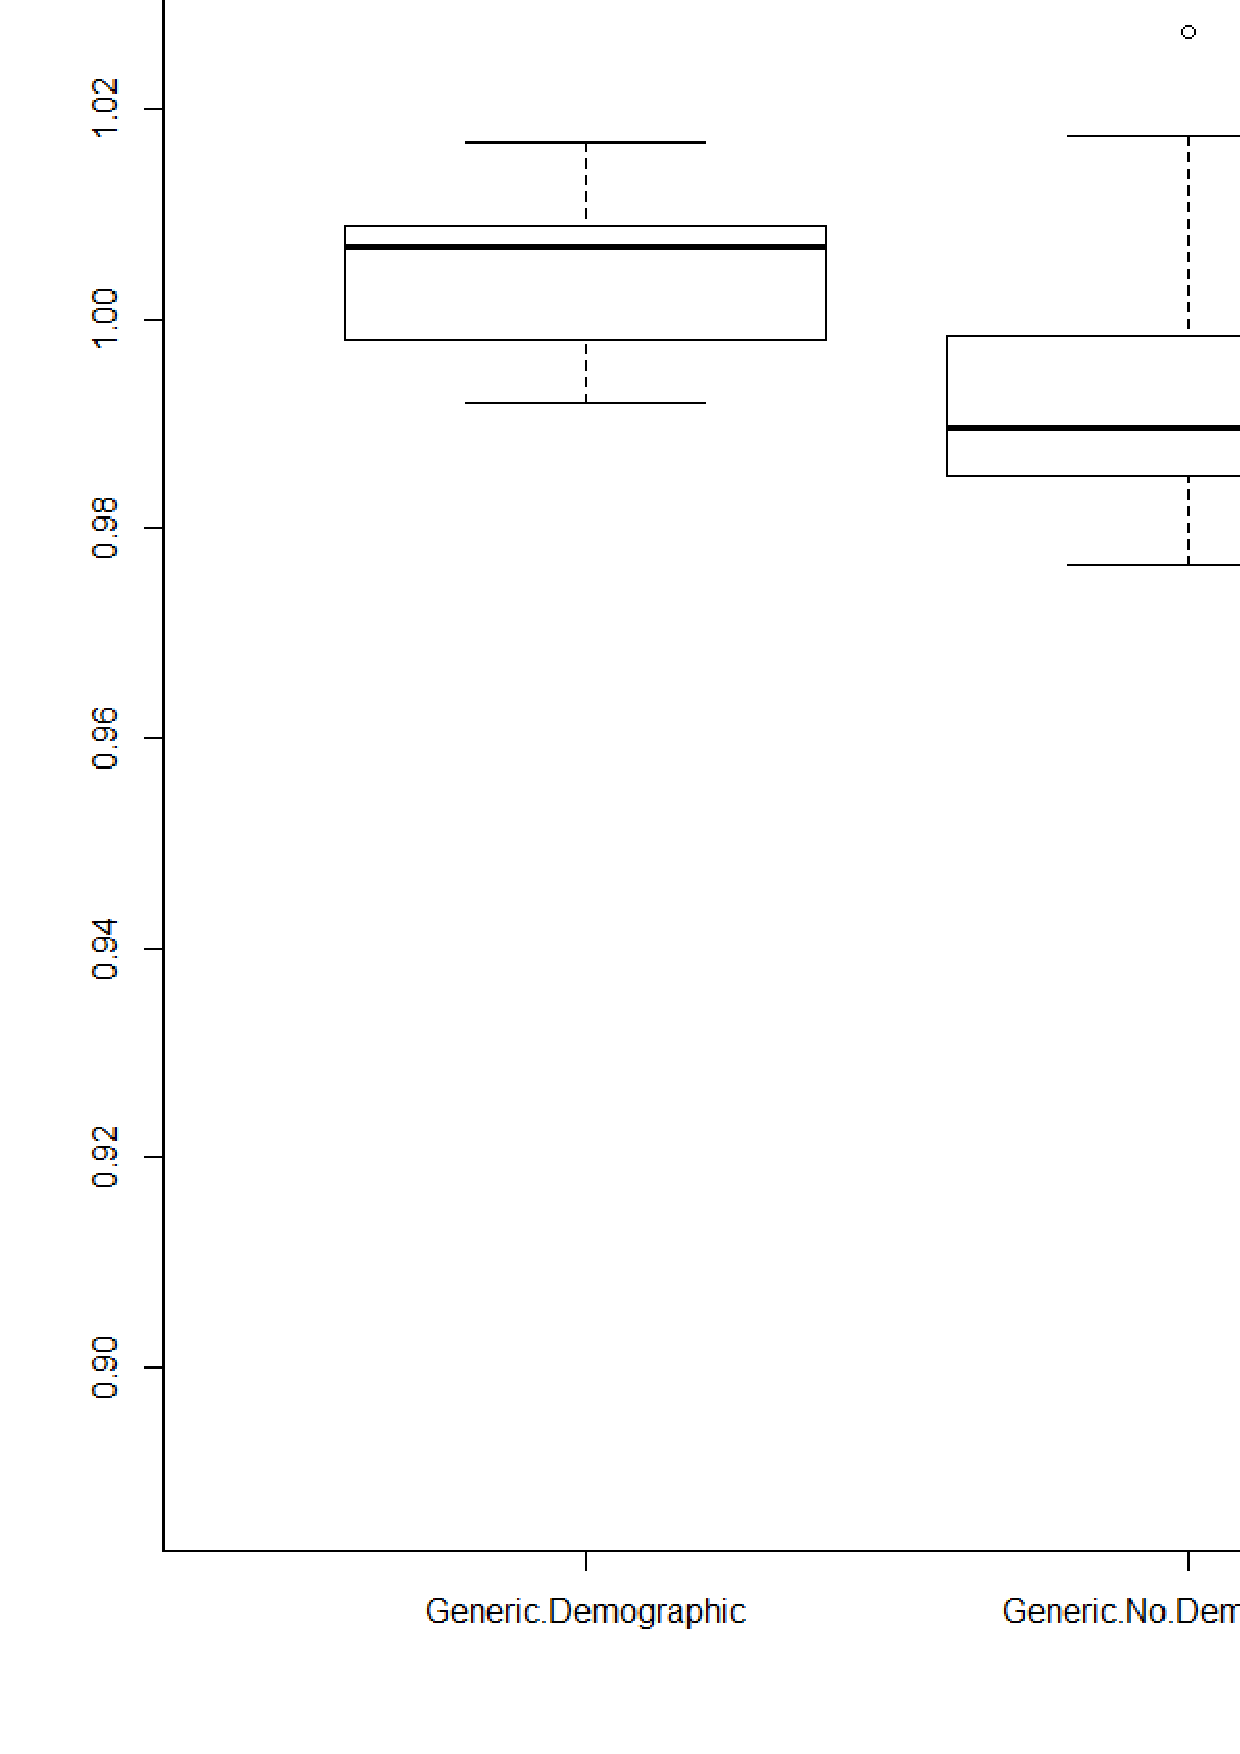
\includegraphics[width=\textwidth]{figs/resultats_10iter.png}
\end{figure}

\begin{figure}[h!]
  \caption{RMSE de diferents variants del SVD i Slope-One.}
  \label{figure-rmse-scores-specific}
  \centering
    \includegraphics[width=\textwidth]{figs/resultats_20iter_specific.png}
\end{figure}

\begin{figure}[h!]
  \caption{Temps tardat en realitzar recomanacions pels diferents sistemes.}
  \label{figure-recommender-speed}
  \centering
    \includegraphics[width=\textwidth]{figs/times.png}
\end{figure}

Donats aquests resultats, el recomanador que anirà millor per a la web seria el SVD, ja que dona bons resultats, i a més a més, és el sistema més ràpid amb bastanta diferència.

\chapter{Conclusions}

\section{Desenvolupament web}

Sobre el desenvolupament de la pàgina web, s'ha desenvolupat una web que és molt senzilla, però que compleix amb l'objectiu, que era donar un frontal per a que l'usuari pugui puntuar pel·lícules, i obtenir recomanacions.

\section{Recomanador}

S'han provat 3 implementacions diferents de recomanadors. S'ha pogut veure que dues d'aquestes (SVD i Slope-One) s'han desmarcat fàcilment del recomanador basat en veïnatge, que es el que s'havia donat al curs, i per tant el que més coneixia i en el que més s'ha treballat.

\section{Possibles ampliacions}

Entre les moltes possibles ampliacions a aquest treball, hi ha dues que mereixen especial menció.

\subsection{Avaluació d'altres paradigmes de recomanació}

Únicament s'ha avaluat un dels paradigmes de la recomanació, que és el filtratge col·laboratiu, per tant encara queda la branca dels recomanadors basats en contingut i dels recomanadors híbrids, que poden donar bastant de joc.

\subsection{Avaluació d'altres recomanadors col·laboratius}

S'han analitzat 3 algoritmes recomanadors, els més coneguts, que son el basat en veïnatge, el Slope-One i el SVD. Es podrien analitzar altres, com per exemple recomanadors basats en xarxes neurals (FALTA CITA) i recomanadors que tinguin en compte quan s'ha realitzat la puntuació (FALTA CITA).

\cleardoublepage
\phantomsection
\addcontentsline{toc}{chapter}{Bibliografia}
\printbibliography
\cleardoublepage

\pagestyle{plain} 
\vspace*{6cm} 
\begin{center} 
\begin{minipage}{4in} 
\parindent=0pt \vspace*{1in} 
\begin{center} 
\vrule width 3in height 0.4pt
\\Firmat:\ Roger Llopart Pla
\\ Bellaterra, 16 de setembre de 2013
\end{center} 
\end{minipage} 
\end{center} 

\newpage 

\thispagestyle{empty}

\vfill{}
{\par\centering \textbf{\large Resum}\large \par}

En aquest treball s'han estudiat diferents sistemes de recomanació, i s'han utilitzat per a veure com podrien arribar a recomanar pel·lícules als usuaris.

Això s'ha realitzat dins del context de la recomanació web, un sistema mitjançant el qual es poden obtenir moltes dades dels usuaris, però que per altra banda requereix de temps de resposta ràpids.

\vfill{}

{\par\centering \textbf{\large Resumen}\large \par}

En este trabajo se han estudiado varios sistemas de recomendación, i se han utilizado para ver como recomendar películas a los usuaris.

Esto se ha llevado a cabo dentro del contexto de la recomendación web, un sistema mediante el cual se pueden obtener muchos datos de los usuarios, pero que por otro lado requiere de tiempos de respuesta rápidos.

\vfill{}

{\par\centering \textbf{\large Abstract}\large \par}

In this study we have evaluated multiple recommender systems, and they've been used to recommend films to users.

This has been done in the context of recomendation on the website. This context allows you to obtain a lot of data about the user, but requires quick response times.

\vfill{}

\end{document}
